% !TEX program = xelatex
% AI-effects 프로젝트 --- 순위 격차 외 지표(누적 점유율, 집중지수·HHI, 탄력성, 로그 거리, 로버스트 z) 엑셀 파일 설명.
% 표 본문: results/table/37_topshare.tex, 37_conc.tex, 37_hhi.tex, 37_elas.tex, 37_dzsum.tex, 37_d_C_ELO.tex, 37_z_C_FEL.tex
%          (code/04_21_analysis_kor_share_exposure_metrics.do가 생성)
% 설명 대상: results/table/37_kor_share_exposure_metrics.xlsx
% 관련: paper 33(같은 정의의 분포 비교, 부트스트랩 구간), 35·36(순위 비교와 순위 격차)
% 컴파일: xelatex -> biber -> xelatex -> xelatex (kotex, biblatex/biber 필요)
\documentclass[11pt]{article}

\usepackage{fontspec}
\usepackage{kotex}
\usepackage[a4paper,margin=2.0cm]{geometry}
\usepackage{longtable}
\usepackage{booktabs}
\usepackage{array}
\usepackage{amsmath}
\usepackage{xcolor}
\usepackage{hyperref}
\usepackage{enumitem}
\usepackage{graphicx}
\usepackage[backend=biber,style=authoryear,maxcitenames=2,uniquelist=false,sorting=nyt]{biblatex}
\addbibresource{../../reference/references.bib}

\hypersetup{colorlinks=true,linkcolor=blue!50!black,urlcolor=blue!50!black}
\newcolumntype{L}[1]{>{\raggedright\arraybackslash}p{#1}}
\newcolumntype{R}[1]{>{\raggedleft\arraybackslash}p{#1}}
\setlength{\LTleft}{0pt}
\setlength{\LTright}{0pt}
\renewcommand{\arraystretch}{1.15}
\setlength{\tabcolsep}{3.5pt}

\title{AI 점유율 지표와 노출도: 순위 격차 외 지표 엑셀 파일 설명\\[2mm]
\large --- 누적 점유율, 집중지수$\cdot$HHI, 탄력성, 로그 거리, 로버스트 $z$ ---}
\author{AI-effects 프로젝트}
\date{\today}

\begin{document}
\maketitle

\begin{abstract}
\noindent 이 노트는 \texttt{results/table/37\_kor\_share\_exposure\_metrics.xlsx}를 설명한다. 파일은 \texttt{code/04\_21\_analysis\_kor\_share\_exposure\_metrics.do}가 만든다. 순위 격차(paper 35$\cdot$36)는 값의 크기와 쏠림을 담지 못하므로, 점유율 지표 A$\cdot$B$\cdot$C와 노출도 3개(Felten AIOE\parencite{felten-2023-how-will-language-modelers-like-chatgpt}, Eloundou $\beta$\parencite{eloundou-2023-gpts-are-gpts-an-early}, Observed Exposure\parencite{massenkoff-2026-labor-market-impacts-of-ai})를 값 자체로 비교하는 지표 다섯 가지를 KSCO 8차 소분류 163개(사용 0인 34개 포함, 2026-11-01)에서 계산했다. 로그를 쓰는 값(로그 거리, 로버스트 z, 탄력성)은 사용 > 0인 129개로 계산한다. 정의는 paper 33과 같고 값도 같다. 이 파일은 그 지표를 직업 목록과 함께 한곳에 정리한 것이다.
\begin{itemize}[leftmargin=*]
  \item \textbf{누적 점유율}: 사용은 상위 10개 소분류가 55\%, 상위 30개가 81$\sim$84\%를 차지한다. 취업자 비중(34\%, 61\%)보다 훨씬 쏠려 있다. 노출도 순으로 줄 세우면 Observed Exposure 상위 10개가 사용의 43\%를, Felten 상위 10개는 7$\sim$8\%만 가진다.
  \item \textbf{집중도}: 노출도 순 집중지수는 0.58$\sim$0.67로 사용이 노출도 높은 직업에 몰려 있다. Observed Exposure로 만든 노출도 기반 점유율(0.64)과는 비슷하고 Eloundou $\beta$(0.37)보다는 크다. 실효 직업 수(1/HHI)는 사용 22개로, 취업자(54개)의 절반이 안 된다.
  \item \textbf{탄력성}: 사용 강도의 Observed Exposure 탄력성은 1.00$\sim$1.07(비례), Eloundou $\beta$ 탄력성은 1.80$\sim$2.21이다. $\beta$의 차이가 사용에서 두 배 가까이 증폭된다.
  \item \textbf{로그 거리와 로버스트 $z$}: 지표 C와 Eloundou $\beta$의 로그 거리는 절댓값 평균 2.21(약 9배 차이)이다. 퍼짐을 맞춘 로버스트 $z$ 차이는 절댓값 평균 0.63$\sim$0.75다. 두 거리 모두에서 213 생명 및 자연과학 관련 시험원이 ``사용 $>$ 노출도'' 1위, 451 조리사가 ``노출도 $>$ 사용'' 1위다.
\end{itemize}
\end{abstract}

\section{파일 구성}

\begin{small}
\begin{longtable}{L{1.7cm}L{3.0cm}L{10.0cm}}
\caption{시트 구성(요청 목록 번호)}\label{tab:sheets}\\
\toprule
시트 & 내용 & 열과 행 \\
\midrule
\endfirsthead
\texttt{topshare} & (1) 누적 점유율 & 분포, 정렬 기준, 상위 10$\cdot$20$\cdot$30개 합(\%). 위 6행은 각 분포를 자기 값 순으로 줄 세운 것(지표 A$\cdot$B$\cdot$C, 노출도 기반 점유율 2개, 참고로 취업자 비중). 아래 12행은 노출도 순으로 줄 세웠을 때 노출도 상위 $k$개 소분류가 가진 사용 점유율(Felten 포함). \\
\texttt{conc} & (2) 집중도 & 왼쪽: 집중지수(사용 지표 $\times$ 노출도 9개, 노출도 기반 점유율 2개). 오른쪽(E열부터): HHI와 실효 직업 수. \\
\texttt{elas} & (3) 탄력성 & 사용 지표 $\times$ 노출도 9행. $\beta$(취업자 가중 OLS)와 robust SE, 95\% 구간, $R^2$, 소분류 수, 비가중 OLS, 분위수 회귀 $\tau = 0.1, 0.5, 0.9$. Felten 행은 준탄력성. \\
\texttt{d\_all} & (4) 로그 거리 & 163개 소분류의 취업자 수, 취업자 비중 $w$, 점유율 $s$, 노출도 기반 점유율 $XS$, 상대 강도 $R$, $RX$, 로그 거리 $d$ 6개. \\
\texttt{d\_top30} & (4) 로그 거리 상위 30 & 쌍(6개) $\times$ 방향(사용 $>$ 노출도, 노출도 $>$ 사용) $\times$ 30행. 열: 사용 지표, 노출도, 방향, 순위, 코드, 직업명, $d$, $e^d$, $R$, $RX$, 취업자 수. \\
\texttt{z\_all} & (5) 로버스트 $z$ & 163개 소분류의 노출도 원값 3개, 로버스트 $z$ 6개, $\Delta z$ 9개. \\
\texttt{z\_top30} & (5) $z$ 차이 상위 30 & 쌍(9개) $\times$ 방향 $\times$ 30행. 열: 사용 지표, 노출도, 방향, 순위, 코드, 직업명, $\Delta z$, $z$(사용), $z$(노출도), 취업자 수. \\
\bottomrule
\end{longtable}
\end{small}

\begin{itemize}[leftmargin=*]
  \item \textbf{``큰 상위 30개''의 뜻}: 로그 거리와 $z$ 차이는 부호가 있다. 절댓값으로 30개를 고르면 두 방향이 섞이므로, 쌍마다 양수 쪽 30개(사용 $>$ 노출도)와 음수 쪽 30개(노출도 $>$ 사용)를 따로 실었다(작업자 판단).
  \item \textbf{Felten}: 음수가 있어 노출도 기반 점유율, 상대 강도, 로그 거리, 탄력성을 만들 수 없다. 순서만 쓰는 누적 점유율(노출도 순)$\cdot$집중지수와 원값으로 만든 로버스트 $z$에는 넣었고, 탄력성 시트에는 원값에 회귀한 준탄력성을 참고로 실었다.
  \item \textbf{사용 0인 34개와 Observed Exposure = 0인 소분류}: 사용 0인 34개는 로그를 쓰는 값(로그 거리, 로버스트 $z$, $\Delta z$, 탄력성)에서 빠진다(129개). 사용이 있으면서 Observed Exposure가 0인 13개는 OE를 쓰는 로그 값($d$(OE), $z$(OE), $\Delta z$(OE), OE 탄력성)에서 더 빠진다(116개). 누적 점유율$\cdot$집중지수$\cdot$HHI는 163개 전부로 계산한다.
\end{itemize}

\section{공통 척도와 정의}

모든 지표는 소분류 163개 안에서 다시 정규화한 같은 척도에서 계산한다(paper 33의 1절과 같다).
\begin{itemize}[leftmargin=*]
  \item 취업자 비중 $w_j = E_j / \sum E$, 사용 점유율 $s^m_j$(합 1, $m$ = A, B, C), 노출도 기반 점유율 $XS^x_j = E_j x_j / \sum_k E_k x_k$($x$ = OE, $\beta$). $XS$는 ``노출도만큼 쓴다면 이 직업이 가졌을 몫''이다.
  \item 상대 강도: 사용 $R^m_j = s^m_j / w_j$, 노출도 $RX^x_j = XS^x_j / w_j = x_j / \bar{x}_E$. 둘 다 취업자 가중 평균이 1이다.
\end{itemize}

\paragraph{(1) 누적 점유율.} 값 내림차순(같은 값은 코드 순; 상위 30 안에는 동점이 없다) 상위 $k$개의 점유율 합이다. 자기 값 순은 그 분포가 얼마나 소수에 몰렸는지를, 노출도 순은 노출도 상위 직업이 실제 사용을 얼마나 가졌는지를 본다.

\paragraph{(2) 집중지수와 HHI.} 집중지수 $\mathrm{CI}(s \mid x) = 1 - 2 \times$(노출도 오름차순으로 취업자 $w$를 누적했을 때 사용 $s$의 누적 곡선 아래 면적)이다. 0이면 사용이 노출도와 무관하게 퍼져 있고, $+1$에 가까울수록 노출도 높은 직업에 몰린다. 같은 노출도는 한 점으로 묶는다. $\mathrm{CI}(XS \mid x)$는 RX의 지니와 같다(do 파일에서 assert). HHI $= \sum s^2$, 실효 직업 수 $= 1/\mathrm{HHI}$는 ``같은 크기의 직업 몇 개에 고르게 나눈 것과 같은 쏠림인가''다.

\paragraph{(3) 탄력성.} $\ln R^m_j = \alpha + \beta \ln RX^x_j$의 $\beta$다. 노출도 강도가 1\% 높을 때 사용 강도가 몇 \% 높은가를 뜻한다. $\beta = 1$이면 사용이 노출도에 비례하고, 1보다 크면 노출도 차이가 사용에서 증폭된다. 주 추정은 취업자 가중 OLS(robust SE)이고, 비가중 OLS와 분위수 회귀를 함께 실었다.

\paragraph{(4) 로그 거리.} $d^{m,x}_j = \ln R^m_j - \ln RX^x_j = \ln(s^m_j / XS^x_j)$다. $e^d$는 ``사용 강도가 노출도 강도의 몇 배인가''이며, paper 29의 로그 비율 LR와 같다.

\paragraph{(5) 로버스트 $z$와 $z$ 차이.} $z(v) = (v - \mathrm{med}(v)) / (1.4826\,\mathrm{MAD}(v))$이고, $v$는 $\ln R^m$, $\ln RX^x$, Felten 원값이다(비가중). $\Delta z = z(\text{사용}) - z(\text{노출도})$는 두 분포의 퍼짐을 맞춘 뒤 ``각자의 분포 안 위치''를 비교한다. 1은 대략 표준편차 하나만큼의 위치 차이다.

\section{결과 개관}

\subsection{누적 점유율}

\begin{small}
\begin{longtable}{L{6.2cm}L{3.6cm}R{1.8cm}R{1.8cm}R{1.8cm}}
\caption{상위 10$\cdot$20$\cdot$30개 누적 점유율(\%)}\label{tab:topshare}\\
\toprule
분포 & 정렬 기준 & 상위 10 & 상위 20 & 상위 30 \\
\midrule
\endfirsthead
% 04_21_analysis_kor_share_exposure_metrics.do가 생성. 직접 고치지 말 것.
지표 A & 자기 값 순 & 54.7 & 71.3 & 81.3 \\
지표 B & 자기 값 순 & 55.5 & 73.9 & 84.1 \\
지표 C & 자기 값 순 & 55.5 & 74.4 & 84.4 \\
노출도 기반 점유율(Observed Exposure) & 자기 값 순 & 56.7 & 76.9 & 85.2 \\
노출도 기반 점유율(Eloundou β) & 자기 값 순 & 43.5 & 62.5 & 74.4 \\
취업자 비중 & 자기 값 순 & 38.3 & 56.5 & 68.2 \\
\midrule
지표 A & Felten AIOE 순 & 6.7 & 33.0 & 39.0 \\
지표 B & Felten AIOE 순 & 7.6 & 34.5 & 41.4 \\
지표 C & Felten AIOE 순 & 8.1 & 35.3 & 41.9 \\
취업자 비중 & Felten AIOE 순 & 3.8 & 9.3 & 15.5 \\
\midrule
지표 A & Eloundou β 순 & 39.1 & 53.8 & 62.8 \\
지표 B & Eloundou β 순 & 38.3 & 53.7 & 62.2 \\
지표 C & Eloundou β 순 & 37.9 & 53.6 & 61.8 \\
취업자 비중 & Eloundou β 순 & 10.9 & 17.0 & 21.7 \\
\midrule
지표 A & Observed Exposure 순 & 43.5 & 56.0 & 66.0 \\
지표 B & Observed Exposure 순 & 43.8 & 56.5 & 66.2 \\
지표 C & Observed Exposure 순 & 43.4 & 56.6 & 66.1 \\
취업자 비중 & Observed Exposure 순 & 5.1 & 16.2 & 21.9 \\

\bottomrule
\end{longtable}
\end{small}

자기 값 순으로 보면 사용 점유율은 상위 10개가 55\%, 상위 30개가 81$\sim$84\%다. 취업자 비중(34\%, 61\%)보다 훨씬 몰려 있다. Observed Exposure로 만든 노출도 기반 점유율도 비슷하게 몰려 있다(56\%, 84\%). Eloundou $\beta$ 기반은 덜하다(41\%, 71\%). $\beta$는 직업 사이 값의 차이가 작아 취업자 분포와 가깝기 때문이다.

노출도 순으로 보면 세 노출도의 성격이 갈린다. Observed Exposure 상위 10개 소분류는 취업자의 4.5\%인데 사용의 43\%를 가진다. Eloundou $\beta$ 상위 10개는 취업자 9\%, 사용 34$\sim$35\%다(사용 0인 853 자동 조립라인 및 산업용로봇 조작원이 5위로 들어 있다). 반면 Felten 상위 10개는 취업자 3\%, 사용 7$\sim$8\%에 그친다. Felten 상위 10에는 교육$\cdot$법률$\cdot$인문 전문가(261, 271, 269, 212)처럼 사용 점유율이 1$\sim$2\%인 직업과 531 통신 관련 판매, 254 종교, 245 영양사, 532 방문 판매처럼 사용이 거의 없는 직업이 섞여 있고, 사용 최상위인 222$\cdot$291은 없다. Felten 상위 20개로 넓히면 291(Felten 12위)과 332(11위)가 들어오면서 사용 몫이 33$\sim$35\%로 크게 늘어난다.

\subsection{집중도}

\begin{longtable}{L{6.4cm}R{2.6cm}R{2.6cm}R{2.6cm}}
\caption{집중지수 CI(노출도 오름차순 누적)}\label{tab:conc}\\
\toprule
분포 & Felten 순 & Eloundou $\beta$ 순 & Observed 순 \\
\midrule
\endfirsthead
% 04_21_analysis_kor_share_exposure_metrics.do가 생성. 직접 고치지 말 것.
지표 A & 0.52 & 0.59 & 0.62 \\
지표 B & 0.55 & 0.62 & 0.63 \\
지표 C & 0.55 & 0.61 & 0.63 \\
\midrule
노출도 기반 점유율(같은 노출도 순) & -- & 0.34 & 0.60 \\

\bottomrule
\end{longtable}

\begin{longtable}{L{8.0cm}R{3.0cm}R{3.0cm}}
\caption{HHI와 실효 직업 수}\label{tab:hhi}\\
\toprule
분포 & HHI & 실효 직업 수 \\
\midrule
\endfirsthead
% 04_21_analysis_kor_share_exposure_metrics.do가 생성. 직접 고치지 말 것.
지표 A & 0.0447 & 22.4 \\
지표 B & 0.0453 & 22.1 \\
지표 C & 0.0455 & 22.0 \\
노출도 기반 점유율(Observed Exposure) & 0.0416 & 24.0 \\
노출도 기반 점유율(Eloundou β) & 0.0282 & 35.5 \\
취업자 비중 & 0.0230 & 43.4 \\

\bottomrule
\end{longtable}

사용의 집중지수는 0.58$\sim$0.67로 모두 양수다. 노출도가 높은 직업일수록 사용 몫이 크다. Observed Exposure 순(0.66$\sim$0.67)이 가장 크고 Felten 순(0.58$\sim$0.61)이 가장 작다. 노출도 기반 점유율과 비교하면, 사용은 Observed Exposure 기반(0.64)과 거의 같은 정도로, Eloundou $\beta$ 기반(0.37)보다는 훨씬 강하게 노출도 쪽에 몰려 있다. 두 비교의 차이가 통계적으로 의미 있는지는 paper 33의 부트스트랩 구간으로 본다(OE와의 차이는 구간이 0을 포함하고, $\beta$와의 차이는 포함하지 않는다).

HHI로 보면 사용 점유율은 실효 직업 수 22개로, 163개 소분류 중 22개에 고르게 나눈 것과 같은 쏠림이다. Observed Exposure 기반(25개)과 비슷하고, Eloundou $\beta$ 기반(39.0개)과 취업자(53.8개)보다 쏠려 있다. 쏠림의 크기가 비슷해도 몰린 직업이 같은 것은 아니다(로그 거리 참고).

\subsection{탄력성}

\begin{footnotesize}
\begin{longtable}{L{1.2cm}L{2.9cm}R{0.9cm}R{0.9cm}R{1.9cm}R{0.8cm}R{0.8cm}R{1.2cm}R{1.0cm}R{1.0cm}R{1.0cm}}
\caption{탄력성 $\ln R = \alpha + \beta \ln RX$(Felten은 원값에 회귀한 준탄력성)}\label{tab:elas}\\
\toprule
사용 & 노출도 & $\beta$ & SE & 95\% 구간 & $R^2$ & $N$ & 비가중 $\beta$ & $\tau$=0.1 & $\tau$=0.5 & $\tau$=0.9 \\
\midrule
\endfirsthead
% 04_21_analysis_kor_share_exposure_metrics.do가 생성. 직접 고치지 말 것.
지표 A & Eloundou β & 1.80 & 0.36 & [1.09, 2.51] & 0.30 & 129 & 2.31 & 1.88 & 2.45 & 2.27 \\
지표 A & Observed Exposure & 1.00 & 0.23 & [0.55, 1.46] & 0.34 & 116 & 0.92 & 1.00 & 0.90 & 1.01 \\
지표 A & Felten AIOE(준탄력성) & 2.18 & 0.38 & [1.42, 2.93] & 0.41 & 129 & -- & -- & -- & -- \\
\midrule
지표 B & Eloundou β & 2.21 & 0.45 & [1.33, 3.10] & 0.32 & 129 & 2.84 & 2.38 & 3.12 & 2.72 \\
지표 B & Observed Exposure & 1.07 & 0.26 & [0.56, 1.58] & 0.30 & 116 & 1.08 & 1.08 & 1.28 & 0.87 \\
지표 B & Felten AIOE(준탄력성) & 2.57 & 0.50 & [1.59, 3.55] & 0.40 & 129 & -- & -- & -- & -- \\
\midrule
지표 C & Eloundou β & 2.16 & 0.44 & [1.28, 3.04] & 0.30 & 129 & 2.80 & 2.18 & 3.25 & 2.73 \\
지표 C & Observed Exposure & 1.06 & 0.27 & [0.53, 1.58] & 0.29 & 116 & 1.08 & 1.10 & 1.12 & 0.94 \\
지표 C & Felten AIOE(준탄력성) & 2.54 & 0.50 & [1.54, 3.54] & 0.39 & 129 & -- & -- & -- & -- \\

\bottomrule
\end{longtable}
\end{footnotesize}

Observed Exposure 탄력성은 1.00$\sim$1.07로, 사용 강도가 노출도 강도에 거의 비례한다. Eloundou $\beta$ 탄력성은 1.80$\sim$2.21이고 95\% 구간이 1을 포함하지 않는다. $\beta$가 평균보다 10\% 높은 직업은 사용 강도가 약 20\% 높다. 비가중 OLS(2.31$\sim$2.84)와 분위수 회귀에서도 $\beta$ 탄력성은 1보다 크다. 즉 $\beta$가 보는 노출도의 차이보다 실제 사용의 차이가 훨씬 크다. Felten 준탄력성은 2.18$\sim$2.57이다(원값 1 증가당 $\ln R$ 증가). $R^2$는 0.29$\sim$0.41로, 노출도가 사용 강도 차이의 3분의 1 남짓만 설명한다.

\subsection{로그 거리}

\begin{small}
\begin{longtable}{R{0.5cm}L{5.0cm}R{2.2cm}L{4.4cm}R{2.4cm}}
\caption{지표 C와 Eloundou $\beta$의 로그 거리 상위$\cdot$하위 10(괄호 = $e^d$)}\label{tab:dCELO}\\
\toprule
 & 사용 $>$ 노출도 & $d$ & 노출도 $>$ 사용 & $d$ \\
\midrule
\endfirsthead
% 04_21_analysis_kor_share_exposure_metrics.do가 생성. 직접 고치지 말 것.
1 & 213 생명 및 자연과학 관련 시험원 & +4.08 (59.1배) & 451 조리사 & -10.81 (1/49423배) \\
2 & 149 기타 건설‧전기 및 생산 관련 관리자 & +4.01 (55.1배) & 611 작물 재배 종사자 & -8.48 (1/4829배) \\
3 & 332 통계‧데이터 관련 사무원 & +3.36 (28.7배) & 872 자동차 운전원 & -7.49 (1/1784배) \\
4 & 122 마케팅 및 광고‧홍보 관리자 & +3.35 (28.4배) & 922 배달원 & -7.19 (1/1329배) \\
5 & 852 냉난방 관련 설비 조작원 & +2.94 (18.9배) & 630 어업 관련 종사자 & -5.97 (1/393배) \\
6 & 298 문화‧예술 관련 기획자 & +2.73 (15.3배) & 952 음식 관련 단순 종사자 & -5.47 (1/237배) \\
7 & 159 기타 판매 및 고객 서비스 관리자 & +2.70 (14.9배) & 864 전기‧전자 부품 및 제품 조립원 & -5.36 (1/213배) \\
8 & 291 작가 및 언론 관련 전문가 & +2.64 (14.0배) & 873 물품 이동 장비 조작원 & -5.22 (1/186배) \\
9 & 292 학예사‧사서 및 기록물 관리사 & +2.60 (13.5배) & 311 기획 및 마케팅 사무원 & -4.71 (1/111배) \\
10 & 223 네트워크 및 정보 보안 전문가 & +2.55 (12.8배) & 244 간호사 & -4.70 (1/110배) \\

\bottomrule
\end{longtable}

\begin{longtable}{L{5.6cm}R{1.6cm}R{1.6cm}R{1.8cm}R{1.8cm}R{1.8cm}}
\caption{지표 C의 거리 요약. $d$ = 로그 거리, $\Delta z$ = 로버스트 $z$ 차이}\label{tab:dzsum}\\
\toprule
항목 & $d$($\beta$) & $d$(OE) & $\Delta z$(Felten) & $\Delta z$($\beta$) & $\Delta z$(OE) \\
\midrule
\endfirsthead
% 04_21_analysis_kor_share_exposure_metrics.do가 생성. 직접 고치지 말 것.
소분류 수 & 129 & 116 & 129 & 129 & 116 \\
10분위 & -4.25 & -3.46 & -1.10 & -0.87 & -1.05 \\
중위값 & -1.00 & -0.07 & 0.18 & 0.35 & 0.12 \\
90분위 & 2.31 & 2.31 & 0.89 & 1.48 & 1.04 \\
절댓값 평균 & 2.21 & 1.88 & 0.63 & 0.75 & 0.68 \\
$|d| > \ln 2$(2배 넘게 차이)인 수 & 108 & 93 & -- & -- & -- \\
$|d| > \ln 10$(10배 넘게 차이)인 수 & 51 & 32 & -- & -- & -- \\
취업자 수와의 Spearman 상관 & -0.57 & -0.64 & -0.50 & -0.38 & -0.49 \\

\bottomrule
\end{longtable}
\end{small}

지표 C와 Eloundou $\beta$의 로그 거리는 절댓값 평균 2.21로, 전형적인 소분류에서 사용 강도와 노출도 강도가 $e^{2.2} \approx 9$배 차이 난다. 사용 > 0인 129개 중 108개가 두 배 넘게, 51개가 열 배 넘게 차이 난다. 위쪽에는 213 생명 및 자연과학 관련 시험원(사용 강도가 노출도 강도의 62배), 149 기타 건설$\cdot$전기 및 생산 관련 관리자(58배), 332 통계$\cdot$데이터 관련 사무원(30배)이 있다. 아래쪽은 451 조리사(약 5만분의 1), 611 작물 재배 종사자, 872 자동차 운전원처럼 사용 점유율이 거의 0인 직업이 차지한다. 로그 거리는 취업자 수와 음의 상관($-0.57$, $-0.64$)이 있다. 큰 직업일수록 사용이 노출도에 못 미친다.

그림~\ref{fig:dbar}은 지표 C $\times$ Eloundou $\beta$ 쌍의 \texttt{d\_top30} 시트를 막대로 그린 것이다. 왼쪽 상위 30은 1.2$\sim$4.1 사이에 고르게 퍼져 있지만, 오른쪽 하위 30은 451 조리사($-10.8$)부터 $-2.8$까지 길게 늘어진다. 로그 거리의 아래쪽 꼬리가 훨씬 긴 것은 사용 점유율이 거의 0인 직업 때문이다(4절 2).
\begin{figure}[htbp]
\centering
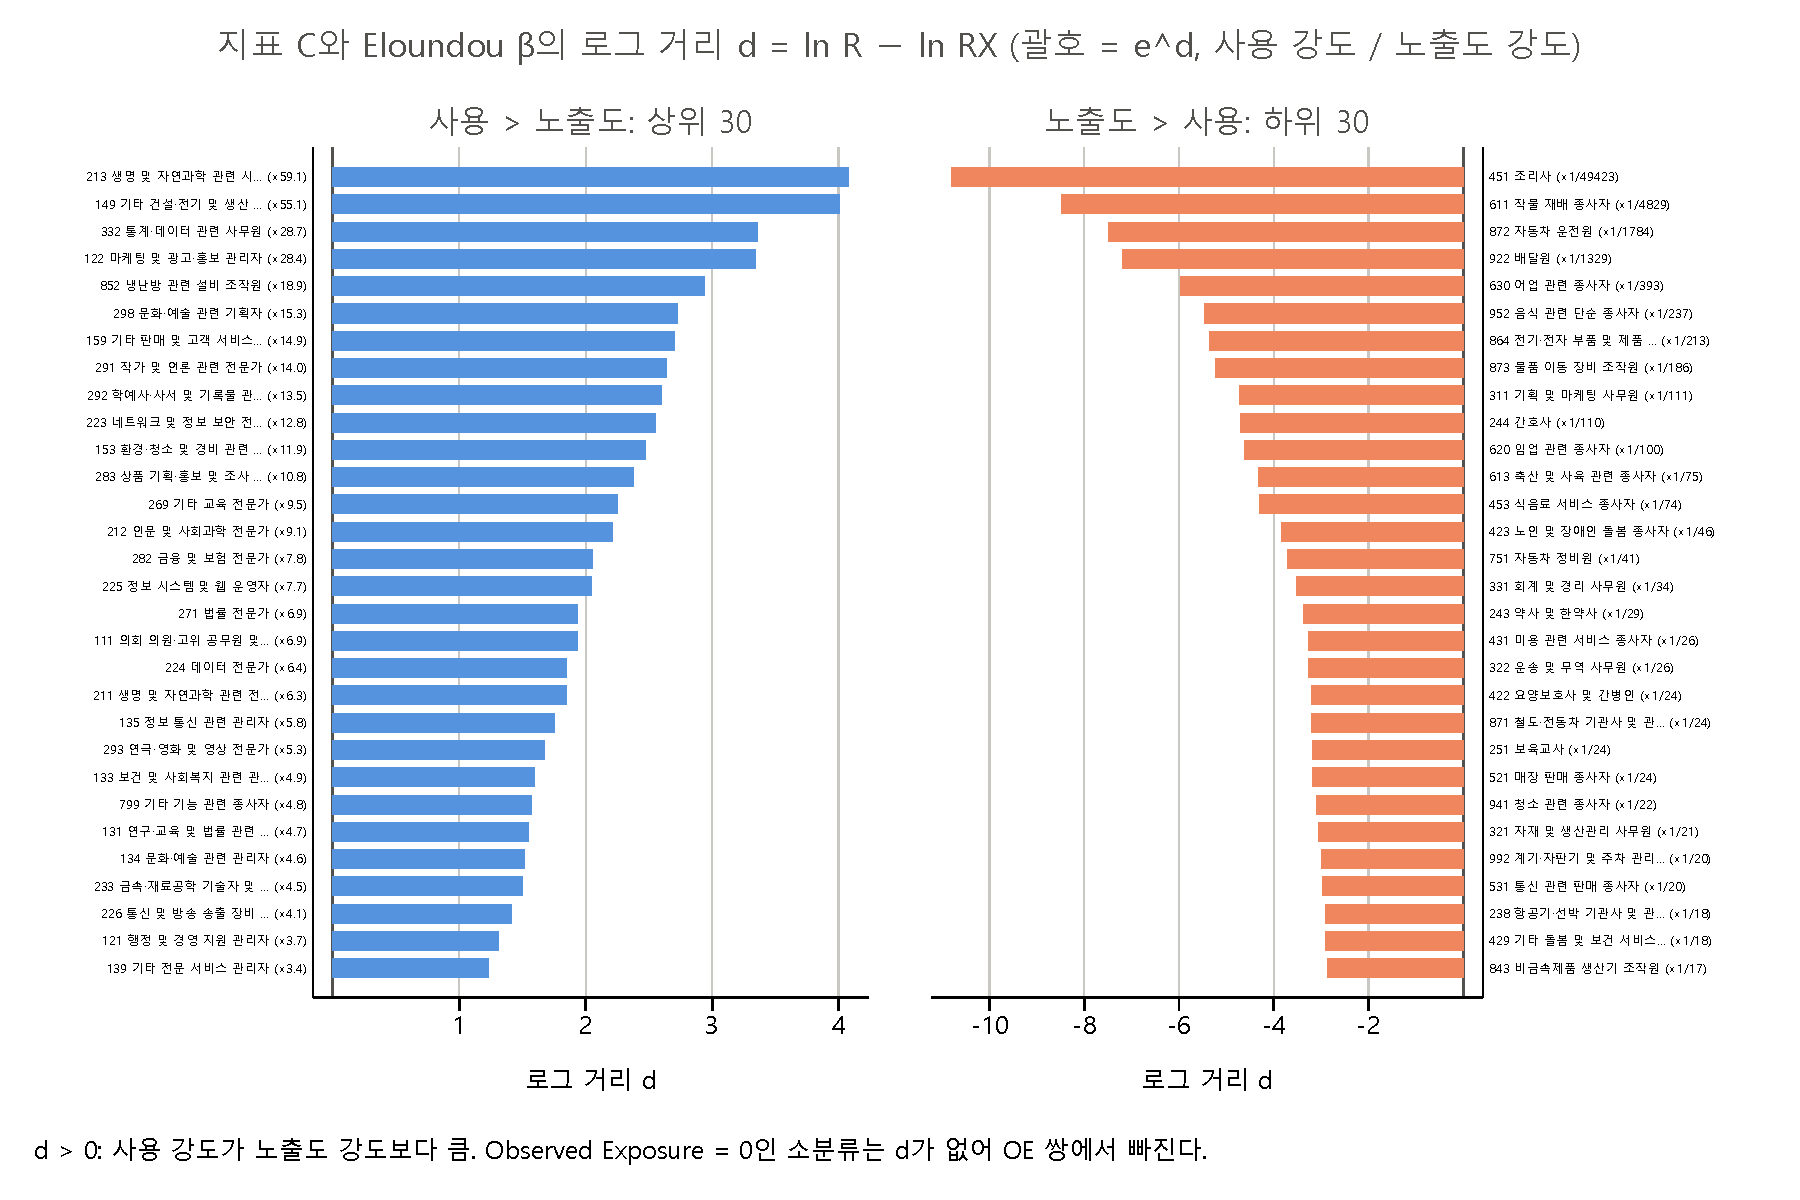
\includegraphics[width=1.0\textwidth]{../figure/37_fig_d_C_ELO_bar.pdf}
\caption{지표 C와 Eloundou $\beta$의 로그 거리 상위 30$\cdot$하위 30(괄호 = $e^d$)}\label{fig:dbar}
\end{figure}


\subsection{로버스트 $z$ 차이}

\begin{small}
\begin{longtable}{R{0.5cm}L{5.4cm}R{1.6cm}L{5.4cm}R{1.6cm}}
\caption{지표 C와 Felten AIOE의 로버스트 $z$ 차이 상위$\cdot$하위 10}\label{tab:zCFEL}\\
\toprule
 & 사용 $>$ 노출도 & $\Delta z$ & 노출도 $>$ 사용 & $\Delta z$ \\
\midrule
\endfirsthead
% 04_21_analysis_kor_share_exposure_metrics.do가 생성. 직접 고치지 말 것.
1 & 213 생명 및 자연과학 관련 시험원 & +2.10 & 451 조리사 & -2.53 \\
2 & 149 기타 건설‧전기 및 생산 관련 관리자 & +1.95 & 531 통신 관련 판매 종사자 & -1.86 \\
3 & 852 냉난방 관련 설비 조작원 & +1.90 & 952 음식 관련 단순 종사자 & -1.67 \\
4 & 799 기타 기능 관련 종사자 & +1.72 & 532 방문 및 노점 판매 종사자 & -1.54 \\
5 & 730 목재‧가구‧악기 및 간판 관련 기능 종사자 & +1.31 & 311 기획 및 마케팅 사무원 & -1.52 \\
6 & 292 학예사‧사서 및 기록물 관리사 & +1.20 & 611 작물 재배 종사자 & -1.52 \\
7 & 791 공예 및 귀금속 세공원 & +1.08 & 245 영양사 & -1.28 \\
8 & 226 통신 및 방송 송출 장비 기사 & +1.08 & 872 자동차 운전원 & -1.22 \\
9 & 882 재활용 처리 및 소각로 조작원 & +0.99 & 322 운송 및 무역 사무원 & -1.20 \\
10 & 225 정보 시스템 및 웹 운영자 & +0.95 & 254 종교 관련 종사자 & -1.20 \\

\bottomrule
\end{longtable}
\end{small}

$\Delta z$는 퍼짐을 맞춘 값이라 로그 거리보다 극단값이 훨씬 작다(절댓값 평균 0.63$\sim$0.75, 표~\ref{tab:dzsum}). 사용 쪽 로그 분산이 노출도 쪽보다 훨씬 커서($\beta$ 기준 약 15배, paper 33), 로그 거리는 사실상 사용 강도의 순서를 따르기 때문이다. $\Delta z$는 그 영향을 빼고 위치만 비교하므로, Felten처럼 로그 거리를 만들 수 없는 노출도도 비교할 수 있다. Felten과의 $\Delta z$ 위쪽에는 213, 149와 함께 852 냉난방 관련 설비 조작원, 799 기타 기능 관련 종사자, 730 목재$\cdot$가구 관련 기능 종사자처럼 Felten이 매우 낮게 매긴 기능직이 들어온다. 아래쪽에는 451 조리사와 함께 531 통신 관련 판매, 532 방문 및 노점 판매, 245 영양사처럼 Felten이 높게 매긴 대면 직업이 있다.

그림~\ref{fig:zbar}는 지표 C $\times$ Felten 쌍의 \texttt{z\_top30} 시트다. 양쪽 모두 절댓값 0.6$\sim$2.5 범위로 비슷하게 퍼져 있어, 로그 거리와 달리 한쪽 꼬리만 길지 않다.
\begin{figure}[htbp]
\centering
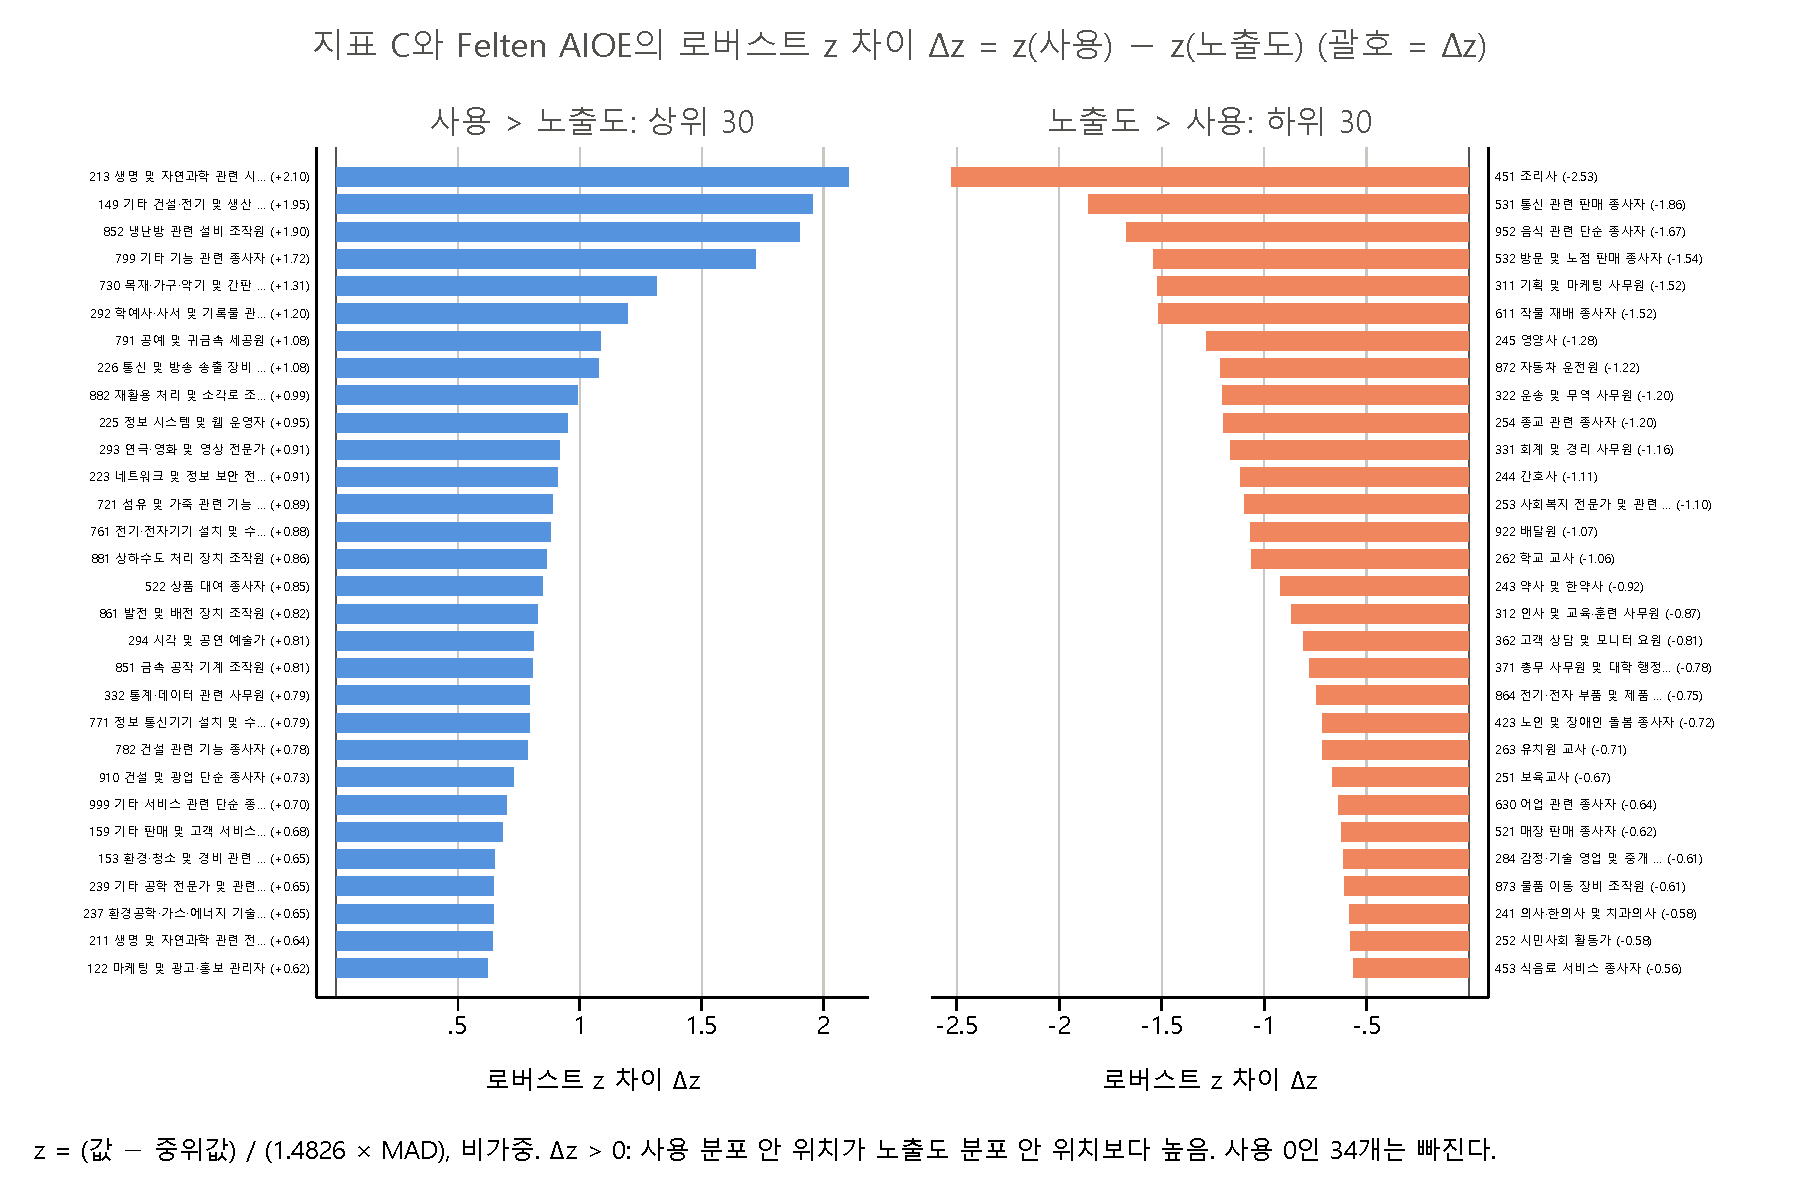
\includegraphics[width=1.0\textwidth]{../figure/37_fig_z_C_FEL_bar.pdf}
\caption{지표 C와 Felten AIOE의 로버스트 $z$ 차이 상위 30$\cdot$하위 30}\label{fig:zbar}
\end{figure}

그림~\ref{fig:dzsc}는 사용 $> 0$인 129개 소분류에서 두 거리를 비교한다. 두 칸 모두 거리는 $y = x$ 선에서 세로로 떨어진 정도다. 왼쪽(로그 거리)은 세로축 $\ln R$($-11\sim4$)이 가로축 $\ln RX$(대부분 $-1.5\sim1$)보다 훨씬 넓어 점들이 거의 세로로 늘어서 있다. 그래서 $d$는 사실상 $\ln R$의 위아래 순서다. 오른쪽($\Delta z$)은 두 축을 각자의 중위값$\cdot$MAD로 맞춰 퍼짐이 비슷하고, 점들이 대각선을 따라 흩어진다. 대각선 위(파랑)는 Felten이 낮게 매긴 기능직(852, 799, 730)이, 아래(주황)는 Felten이 높게 매긴 판매$\cdot$사무 직업(531, 532, 311)이 차지한다.
\begin{figure}[htbp]
\centering
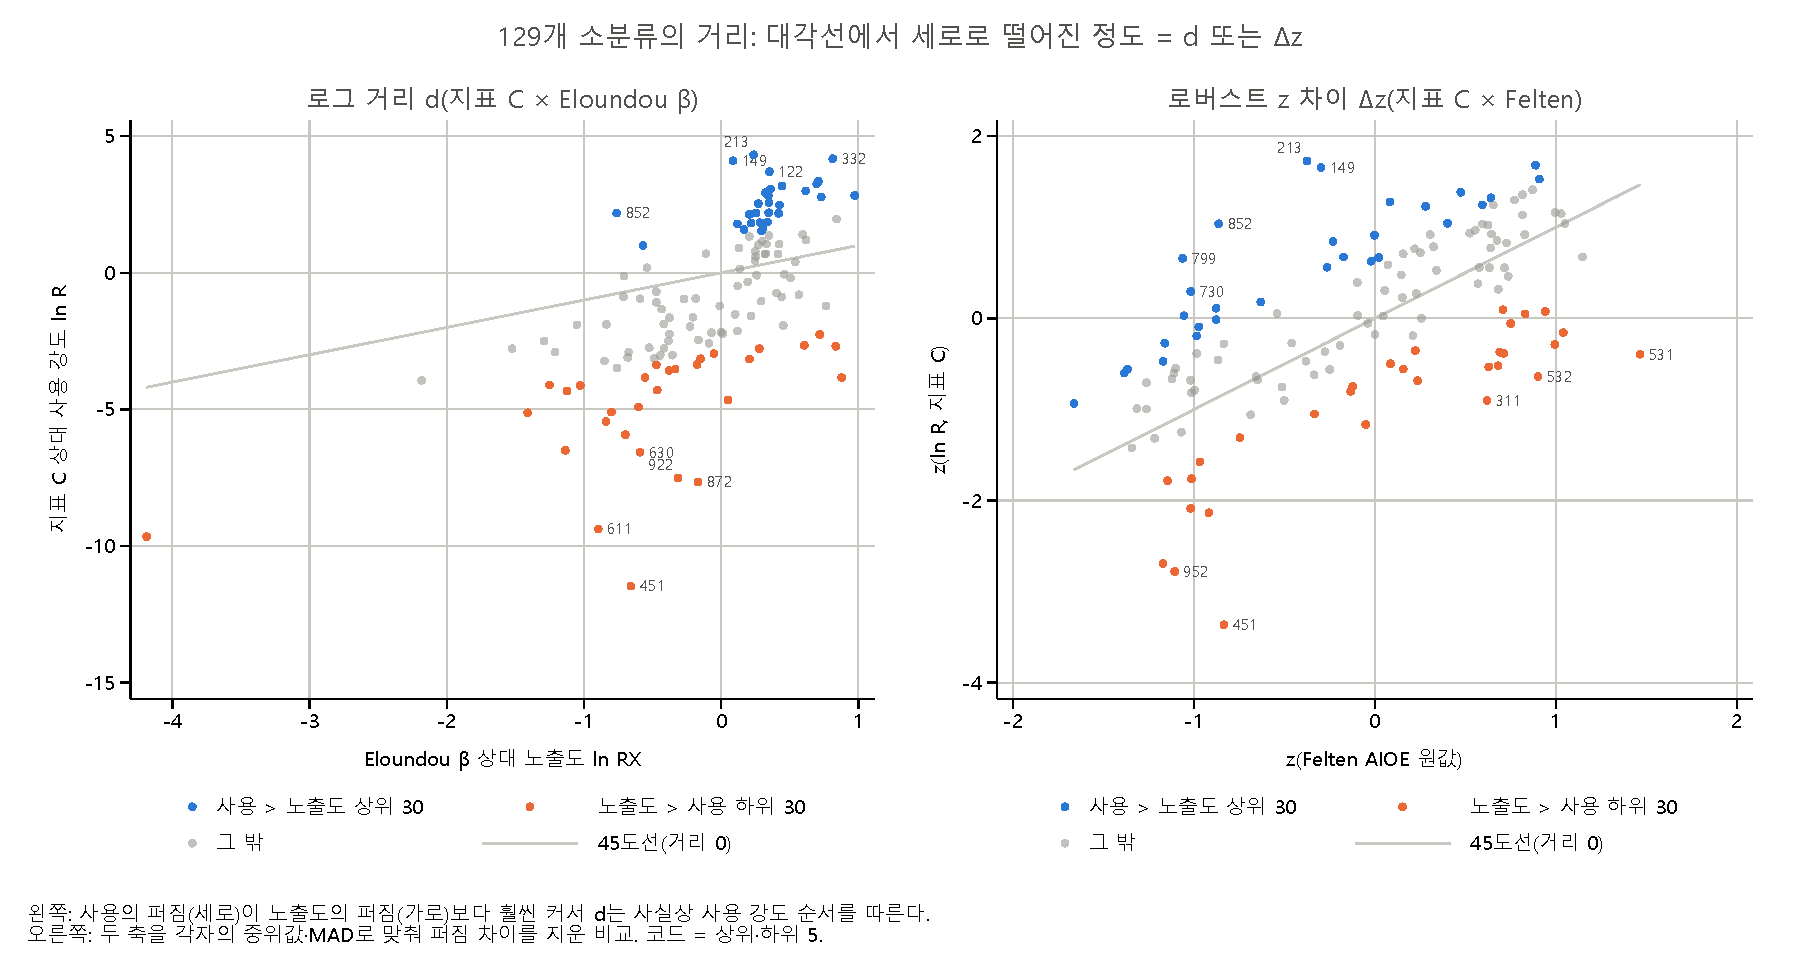
\includegraphics[width=1.0\textwidth]{../figure/37_fig_dz_scatter.pdf}
\caption{사용 $> 0$인 129개 소분류의 로그 거리(왼쪽)와 로버스트 $z$ 차이(오른쪽): $y = x$ 선에서 세로 거리 = $d$ 또는 $\Delta z$}\label{fig:dzsc}
\end{figure}


\section{읽을 때 유의사항}

\begin{enumerate}[leftmargin=*]
  \item \textbf{paper 33과 같은 값이다.} 정의와 표본이 같아 수치가 일치한다. 부트스트랩 신뢰구간과 대분류 분해는 paper 33에 있고, 이 파일에는 탄력성의 해석적(robust SE) 구간만 실었다.
  \item \textbf{로그 거리의 아래쪽 끝은 불안정하다.} 사용 점유율이 거의 0인 소분류는 $d$가 $-5\sim-11$까지 내려간다. 451$\cdot$611$\cdot$952처럼 한 달만 공개된 소분류가 많고, 이들은 비공개 달을 0으로 둔 영향으로 값이 절반이다. 이 끝은 $\Delta z$와 함께 읽는다.
  \item \textbf{$\Delta z$는 ``몇 배''가 아니다.} 각자의 분포 안 위치 차이이며, 0도 ``사용 = 노출도''가 아니라 ``두 분포에서 같은 상대 위치''다. 비가중이므로 취업자 가중 통계(집중지수, 탄력성)와 직접 맞대지 않는다. Felten은 원값, 나머지는 로그 상대 강도로 $z$를 만들었으므로 Felten과 다른 노출도의 $\Delta z$를 같은 눈금으로 비교하는 것은 근사다.
  \item \textbf{점유율은 직업 규모가 들어간 값이다.} 누적 점유율$\cdot$HHI는 큰 직업의 영향을 받는다. 상대 강도($R$, $RX$)와 그 위의 지표(탄력성, 로그 거리, $\Delta z$)는 규모를 뺀 비교다.
  \item \textbf{두 쪽 모두 SOC 값을 연계표로 옮긴 것이다}(paper 21, 23). 한 SOC에 쏠린 소분류는 그 SOC의 값에 따라 거리가 크게 움직인다.
\end{enumerate}

\section{산출 파일}

\begin{itemize}[leftmargin=*]
  \item 코드: \texttt{code/04\_21\_analysis\_kor\_share\_exposure\_metrics.do}(Stata 17, \texttt{00\_master.do}에 포함). 입력은 \texttt{data/proc/merged/kor\_ai\_usage\_ksco3.dta}(\texttt{03\_05}). 확인하는 항등식: 상대 강도의 취업자 가중 평균 1, $d = \ln(s / XS)$, CI($XS^x \mid x$) = 지니($RX^x$).
  \item 엑셀: \texttt{results/table/37\_kor\_share\_exposure\_metrics.xlsx}(시트 7개).
  \item 이 노트의 표: \texttt{results/table/37\_topshare.tex}, \texttt{37\_conc.tex}, \texttt{37\_hhi.tex}, \texttt{37\_elas.tex}, \texttt{37\_d\_C\_ELO.tex}, \texttt{37\_dzsum.tex}, \texttt{37\_z\_C\_FEL.tex}.
  \item 그림: \texttt{results/figure/37\_fig\_d\_C\_ELO\_bar}, \texttt{37\_fig\_z\_C\_FEL\_bar}, \texttt{37\_fig\_dz\_scatter}(각 \texttt{.pdf}, \texttt{.png}; 같은 do 파일이 생성).
\end{itemize}

\printbibliography[title={참고문헌}]

\end{document}
